% !TEX program = xelatex
% 编译方式：xelatex 连续编译两遍（以正确生成 longtable 跨页与目录）。
\documentclass[12pt,a4paper]{ctexart}

\usepackage{amsmath,amssymb,bm}
\usepackage{geometry}
\geometry{left=2.5cm,right=2.5cm,top=2.5cm,bottom=2.5cm}
\usepackage{booktabs}
\usepackage{longtable}
\usepackage{array}
\usepackage{multirow}
\usepackage{enumitem}
\usepackage{caption}
\usepackage{float}
\usepackage{xcolor}
\usepackage{listings}
\usepackage{fancyhdr}
\usepackage{graphicx}

\captionsetup{font=small,labelsep=quad}
\renewcommand{\arraystretch}{1.25}

\lstset{
  basicstyle=\ttfamily\small,
  keywordstyle=\color{blue!70!black}\bfseries,
  commentstyle=\color{green!45!black},
  stringstyle=\color{orange!80!black},
  numbers=left,
  numberstyle=\tiny\color{gray},
  stepnumber=1,
  breaklines=true,
  breakatwhitespace=false,
  columns=fullflexible,
  keepspaces=true,
  showstringspaces=false,
  frame=single,
  rulecolor=\color{gray!50},
  tabsize=4,
  language=Python,
  extendedchars=true
}

\pagestyle{fancy}
\fancyhf{}
\rhead{\small 多工序协同作业下的车间整修调度与资源分配}
\lfoot{}\rfoot{\thepage}
\renewcommand{\headrulewidth}{0.4pt}

\title{\bfseries 多工序协同作业下的车间整修任务调度与资源分配优化}
\author{}
\date{}

\begin{document}
\maketitle
\thispagestyle{fancy}

%==================================================================
\begin{center}
\textbf{摘要}
\end{center}

本文围绕多工序协同作业环境下的车间整修任务调度与资源分配优化问题，基于组合优化与约束规划理论，建立了统一的工序链—资源—转运网络模型，系统研究了从单车间到多车间、从单班组到双班组及从固定资源配置到预算约束下资源购置决策等不同场景下的最优调度方案。本文全部数学模型的计算与模拟过程均通过 Python 编程实现（基于 OR-Tools CP-SAT 求解器及自编遗传算法与模拟退火程序），确保了算法的可执行性与结果的可复现性。

针对问题一，本文在单车间串行结构下，基于工序严格串行与同类设备并行分担工程量的核心机理，通过解析计算确定班组 1 完成 A 车间全部工序的最短时长。由于 A 车间仅含三道工序且无跨车间竞争，瓶颈完全由单台设备工序决定，通过投入全部可用台数并行分担协同工序工程量，解析求得最短完工时间为 $37280\,\mathrm{s}$，并给出了每台设备的作业时间线。

针对问题二，将场景扩展至班组 1 独立完成 A、B、C、D、E 五个车间的全部整修任务，构建了带序列相关转移时间与协同加工约束的资源受限车间调度整数规划模型。以最小化总完工时间为目标，引入路由变量刻画各类设备在工序间的访问顺序，采用大 $M$ 法建立资源析取与跨车间转运约束。提出遗传算法与模拟退火级联生成可行上界、以 \texttt{AddHint} 热启动注入 CP-SAT 求解器的两层混合求解框架，由约束规划完成零间隙最优性证明，得到最短完工时间为 $144880\,\mathrm{s}$。

针对问题三，在问题二模型基础上引入班组 2 设备，将两班组同类设备合并为统一资源池，模型结构不变而资源容量翻倍，初始转运取两基地到各车间的较大值。求解得到最短完工时间为 $73575\,\mathrm{s}$，较问题二缩短约 $49.2\%$，接近资源翻倍的理想加速比。

针对问题四，在双班组基础上追加总额 $500000$ 元的设备购置预算，构建了购置—调度耦合的双层优化模型。外层以资源载荷下界分析将购置维度由五类设备严格降至高速抛光机与自动传感多功能机两类瓶颈设备，枚举可行购置组合；内层对每个组合调用混合求解框架精确求解。得到最优购置方案为增购高速抛光机与自动传感多功能机各 3 台（费用 $465000$ 元），最短完工时间为 $32608\,\mathrm{s}$，较问题三缩短约 $55.7\%$。冷启动与热启动对比实验表明，\texttt{AddHint} 热启动使 CP-SAT 求解耗时加速约 $1.4\times$--$2.1\times$。

\noindent\textbf{关键字：}\,作业车间调度；序列相关转移时间；混合求解；约束规划；遗传算法；模拟退火

%==================================================================
\section{问题分析}

四个子问题在规模与决策维度上层层递进：从单车间到五车间、从单班组到双班组、从固定配置到预算约束下的购置决策。本文据此设计统一的建模框架，使各问的模型在结构上保持一致、在能力上逐步增强。

\subsection{问题一的分析}

问题一要求仅使用班组 1 的设备完成 A 车间的全部整修任务，计算最短完工时长并给出每台设备的作业调度明细。A 车间含 A1（精密灌装机与自动化输送臂协同，$300\,\mathrm{m}^3$）、A2（高速抛光机与工业清洗机协同，$500\,\mathrm{m}^3$）、A3（自动传感多功能机，$500\,\mathrm{m}^3$）三道严格串行工序。由于仅涉单一车间，无跨车间设备竞争与转运，决策自由度仅在于同类多台设备是否全部投入协同工序的工程量分担。问题规模小、结构简单，可通过解析方式直接求得最优解，无需借助一般调度框架。该问题同时为后续多车间调度确立工时计算口径与可分负载假设。

\subsection{问题二的分析}

问题二要求仅使用班组 1 的设备，同时完成 A、B、C、D、E 五个车间的整修任务，其中 C 车间的 C3--C5 工序需重复三遍。此时间题升级为带序列相关转移时间与协同加工约束的多机作业车间调度：每个车间为一条固定工序链，每道工序占用一种或两种设备类型，同类设备全局串行服务，跨车间切换须预留转运时间。与经典柔性作业车间调度问题（FJSP）的差异在于：协同工序的工期由两类设备中较慢者决定，转移时间取决于设备前一作业车间与下一作业车间的距离，同类多台设备可并行分担工程量从而缩短单工序占用时间。本文对同类设备建立聚合抽象（超级机器），将问题建模为每类设备在工序间的路由选择与时间排程问题，设计元启发式生成上界、约束规划精确证明的两层混合求解策略。

\subsection{问题三的分析}

问题三在问题二的基础上引入班组 2 的设备资源。两班组所配备的设备类型完全相同（五类设备各若干台），故自然地将同类设备合并为统一资源池：自动化输送臂增至 8 台、工业清洗机与精密灌装机各增至 10 台、自动传感多功能机与高速抛光机各增至 2 台。模型结构与问题二完全一致，仅资源容量参数与初始转运参数（取两基地到各车间转运时间的最大值）发生变化，体现了建模框架的可扩展性。由于瓶颈资源（高速抛光机、自动传感多功能机）翻倍，预期总工期将有显著下降。

\subsection{问题四的分析}

问题四在问题三的双班组资源池基础上，追加总额为 $500000$ 元的设备购置预算，需联合确定购置方案与调度策略使总完工时间最短。该问题构成购置—调度耦合的双层优化：外层决定增购哪些设备、各增购多少台，内层在给定设备配置下求解最优调度。五类设备均可增购，若直接枚举组合则搜索空间过大。本文利用资源载荷下界分析识别瓶颈设备，论证只有增购当前瓶颈设备才可能降低总工期下界，从而将外层搜索空间由五维压缩至二维（仅高速抛光机与自动传感多功能机），使枚举所有可行购置组合成为可能。

%==================================================================
\section{模型假设}
\begin{enumerate}[label=(\arabic*),leftmargin=2.2em]
\item 各车间内部工序顺序固定，必须严格按给定编号由小到大依次执行，前序工序完工后后序工序方可开工；C 车间的 C3\,--\,C5 工序按题意重复三遍。
\item 当一道工序需两类设备协同完成时，两类设备各自独立完成该工序对应的全部工程量，二者之间不计先后顺序与相互等待；当且仅当两类设备均完成其工程量时该工序判定完工，故工序工期取两类设备作业时间的较大者，而非求和或取较小者。
\item 同一类设备的多台机器可并行分担同一工序的工程量（可分负载），分担后各机器作业时间相等，工序的该类设备作业时间为工程量除以该类设备总作业效率。
\item 各班组设备数量固定，设备可在不同工序间重复使用，但同一时刻每台物理设备至多服务一道工序。
\item 转运按单台物理设备独立计取：题目假定“同一台设备”跨车间转移须计入运输时间，$\tau_{w,w'}=\lceil d_{w,w'}/2\rceil$（s），与同类其他设备是否同时移动无关；同一台设备在同一车间不同工序间的转移时间忽略不计。
\item 在资源池化/编组作业口径下，同类 $n_r$ 台设备在同一工序上并行作业、在同一时刻切换至下一作业车间时，各台设备并行转场，日历时间仅增加一次 $\tau_{w,w'}$，而非按台数累加；该处理与单台独立移动、速度相同相容，亦不同于将多类设备绑定的整车运输。
\item 计时自 $00{:}00{:}00$ 起，设备可在零时刻自所属班组基地出发；首道作业须计入由基地到该车间的初始转运。双班组情形下，编组首达时刻取 $\max_{b\in\mathcal{B}}\tau_{b,w}$。
\item 设备性能稳定，作业过程不发生故障与中断，转运速度恒为 $2\,\mathrm{m/s}$；所有持续工作时间精确到秒且向上取整。
\end{enumerate}

%==================================================================
\section{符号说明}
\begin{longtable}{p{3.2cm} p{11.5cm}}
\toprule
\textbf{符号} & \textbf{含义} \\
\midrule
\endfirsthead
\toprule
\textbf{符号} & \textbf{含义} \\
\midrule
\endhead
\bottomrule
\endfoot
$W$ & 车间集合，$W=\{A,B,C,D,E\}$ \\
$\mathcal{O}_w$ & 车间 $w$ 的有序工序序列（含 C 车间三遍循环展开） \\
$\mathcal{O}$ & 全部工序集合，$\mathcal{O}=\bigcup_{w\in W}\mathcal{O}_w$ \\
$o,o'$ & 工序索引；$w(o)$ 表示工序 $o$ 所属车间 \\
$\mathcal{R}$ & 设备类型集合 $\{$输送臂, 清洗机, 灌装机, 传感机, 抛光机$\}$ \\
$n_r$ & 类型 $r$ 设备的可用台数 \\
$\mathcal{R}(o)$ & 工序 $o$ 所需的设备类型集合（含一类或两类） \\
$v_o$ & 工序 $o$ 的工程量（$\mathrm{m}^3$） \\
$e_{o,r}$ & 类型 $r$ 设备在工序 $o$ 的单台作业效率（$\mathrm{m}^3/\mathrm{h}$） \\
$p_{o,r}$ & 类型 $r$ 完成工序 $o$ 的作业时间，$p_{o,r}=\lceil v_o/(e_{o,r}\,n_r)\cdot 3600\rceil$（s） \\
$p_o$ & 工序 $o$ 的工期，$p_o=\max_{r\in\mathcal{R}(o)} p_{o,r}$（s） \\
$d_{w,w'}$ & 车间（或基地）$w$ 与 $w'$ 间距离（m） \\
$\tau_{w,w'}$ & 由 $w$ 到 $w'$ 的转运时间，$\tau_{w,w'}=\lceil d_{w,w'}/2\rceil$（s）；按单台物理设备计取 \\
$\tau^{\mathrm{init}}_{w}$ & 编组首达车间 $w$ 的初始转运，$\max_{b\in\mathcal{B}}\tau_{b,w}$ \\
$s_o,\;f_o$ & 工序 $o$ 的开工时刻与完工时刻，$f_o=s_o+p_o$ \\
$x^{r}_{o,o'}$ & 路由变量，类型 $r$ 上工序 $o$ 紧邻于 $o'$ 之前时取 $1$ \\
$C_{\max}$ & 总完工时间（makespan） \\
$B$ & 设备购置预算，$B=500000$ 元 \\
$c_r,\;z_r$ & 类型 $r$ 设备单价与增购台数 \\
\end{longtable}

%==================================================================
\section{问题一：单链可分负载分配模型}

\subsection{问题分析与建模}
问题一假定班组 1 独立整修 A 车间。A 车间含三道严格串行工序：A1（精密灌装机与自动化输送臂协同，$300\,\mathrm{m}^3$）、A2（高速抛光机与工业清洗机协同，$500\,\mathrm{m}^3$）、A3（自动传感多功能机，$500\,\mathrm{m}^3$）。由于工序串行、无跨车间竞争（仅首道计入 $\tau_{\mathrm{G1},A}$），可优化自由度仅为同类设备并行分担的程度。

若类型 $r$ 投入 $k$ 台机器分担工序 $o$，则
$p_{o,r}(k)=\lceil v_o/(e_{o,r}k)\cdot 3600\rceil$ 关于 $k$ 单调不增，故每道工序对每类所需设备均投入全部可用台数 $n_r$ 最优。对协同工序，由假设 (2)，
\begin{equation}
p_o=\max_{r\in\mathcal{R}(o)}p_{o,r}(n_r),\qquad
C_{\max}^{(1)}=\tau_{\mathrm{G1},A}+\sum_{o\in\mathcal{O}_A}p_o.
\end{equation}
以 A1 为例，灌装机与输送臂分别得 $1080\,\mathrm{s}$，故 $p_{A1}=1080\,\mathrm{s}$，而非 $2160\,\mathrm{s}$（求和）或取较小者。A2 中抛光机单台得 $18000\,\mathrm{s}$、清洗机五台并行得 $1440\,\mathrm{s}$，故 $p_{A2}=18000\,\mathrm{s}$；$p_{A3}=18000\,\mathrm{s}$。于是 $C_{\max}^{(1)}=200+1080+18000+18000=37280\,\mathrm{s}$。瓶颈来自单台高速抛光机与单台自动传感多功能机。详细调度见表~\ref{tab:q1}。

%==================================================================
\section{问题二：单班组聚合作业车间调度模型}

\subsection{问题结构辨识}
问题二在单班组配置下同时整修五个车间，决策包括各工序开工时刻、各类型设备在工序间的访问顺序及由此诱导的跨车间转运。其结构为带序列相关转移时间（SDST）与协同加工约束的多机作业车间调度：每个车间为固定工序链；每道工序占用一种或两种设备类型；同一类型设备在聚合口径下全局串行服务，跨车间切换须预留转运时间。与经典 FJSP 的差异在于：协同工序工期由较慢者决定；转移时间取决于设备上一作业车间与下一作业车间；同类多台设备可并行分担工程量从而改变 $p_{o,r}$。

\subsection{工时参数推导}
对工序 $o$、类型 $r\in\mathcal{R}(o)$，在池化台数 $n_r$ 下，
\begin{equation}
p_{o,r}=\left\lceil\frac{v_o}{e_{o,r}\,n_r}\cdot 3600\right\rceil,\qquad
p_o=\max_{r\in\mathcal{R}(o)}p_{o,r},\quad f_o=s_o+p_o.
\end{equation}
式 (2) 体现双设备各自完成全部工程量、以较晚者完工的题设；类型 $r$ 仅占用 $[s_o,s_o+p_{o,r}]$，若 $p_{o,r}<p_o$ 则可提前释放。若将 $p_o$ 误取为求和或单类时长，将破坏资源占用与工序链的一致性。

\subsection{资源聚合、转运机理与抽象边界}
若对每一台物理设备单独建立路由，决策规模将急剧膨胀，且与瓶颈结构（单台抛光机、单台传感机）不相称。由假设 (3)，将类型 $r$ 的 $n_r$ 台设备聚合为容量 $n_r$ 的超级机器，在工序 $o$ 上占用 $p_{o,r}$。

\textbf{转运口径}：按假设 (5)--(6)，转运由单台物理设备独立完成。在编组作业方案中，当类型 $r$ 由车间 $w$ 的工序 $o$ 切换至车间 $w'$ 的工序 $o'$ 时，各物理设备并行转场，日历约束为
$s_{o'}\ge s_o+p_{o,r}+\tau_{w,w'}$（$w\neq w'$）。
该式不是整车运输（多类设备捆绑），亦非逐台串行运输（否则将误乘 $n_r$）；在速度相同、目标相同的前提下，并行转场的日历延迟与单台转场相同。对 $n_r=1$ 的瓶颈资源，聚合与个体建模在转运维度等价。

聚合假设同类设备遵循同一访问序列，不允许同类设备分赴不同车间并行服务不同工序；该简化对非瓶颈类型可能略偏保守，但不改变本题主导结论。

\subsection{整数规划模型}
记 $\mathcal{O}(r)=\{o\in\mathcal{O}:r\in\mathcal{R}(o)\}$（类型 $r$ 需要服务的全部工序集合），引入路由变量 $x^{r}_{o,o'}\in\{0,1\}$，当类型 $r$ 在完成工序 $o$ 后立即转至工序 $o'$ 时取 $1$；引入虚拟节点 $0$ 表示班组基地（出发与返回均为同一基地）。模型如下：
\begin{align}
\min~~ & C_{\max} \label{eq:obj}\\
\text{s.t.}~~ & f_o = s_o + p_o, \quad \forall o\in\mathcal{O}, \label{eq:def}\\
& s_{o'} \ge f_o, \quad \forall w,\ \forall (o,o')\in\mathcal{P}(\mathcal{O}_w), \label{eq:prec}\\
& s_{o'} \ge s_o + p_{o,r} + \tau_{w(o),w(o')} - M\,(1-x^{r}_{o,o'}), \quad \forall r,\ o\neq o'\in\mathcal{O}(r), \label{eq:disj}\\
& \textstyle\sum_{o'\in\mathcal{O}(r)} x^{r}_{0,o'} = 1,\quad \sum_{o\in\mathcal{O}(r)} x^{r}_{o,0}=1, \quad \forall r, \label{eq:flow}\\
& \texttt{AddCircuit}\big(\{(o,o')\mid x^{r}_{o,o'}=1\}\big), \quad \forall r, \label{eq:circuit}\\
& s_o \ge \tau^{\mathrm{init}}_{w(o)} - M\,(1-x^{r}_{0,o}), \quad \forall r,\ o\in\mathcal{O}(r), \label{eq:init}\\
& C_{\max} \ge f_o, \quad \forall o\in\mathcal{O}, \label{eq:cmax}\\
& s_o\ge 0,\quad f_o\ge 0,\quad x^{r}_{o,o'}\in\{0,1\}, \quad \forall r,\ o,o'\in\mathcal{O}(r)\cup\{0\}. \notag
\end{align}
其中 $\mathcal{P}(\mathcal{O}_w)$ 表示车间 $w$ 的工序链 $\mathcal{O}_w$ 中所有相邻工序对构成的集合；$\texttt{AddCircuit}$ 为 OR-Tools CP-SAT 求解器内置的回路约束，强制变量 $\{x^{r}_{o,o'}\}$ 构成一条从虚拟节点 $0$（基地）出发、遍历 $\mathcal{O}(r)$ 中每道工序恰好一次并返回 $0$ 的哈密顿回路；$\tau^{\mathrm{init}}_{w}=\max_{b\in\mathcal{B}}\tau_{b,w}$（取各基地到车间 $w$ 转运时间的最大值），问题二只有班组 1，故 $\mathcal{B}=\{\mathrm{G1}\}$，$\tau^{\mathrm{init}}_{w}=\tau_{\mathrm{G1},w}$；$M$ 为充分大的常数，本文取时间上界 $H$（所有工序工期之和加冗余），即当路由弧未激活（$x^{r}_{o,o'}=0$）时使对应不等式自动松弛。

\medskip
\noindent 各约束的含义逐条解释如下：

\begin{enumerate}[leftmargin=2.2em, label=(\arabic*)]
\item \textbf{目标函数 \eqref{eq:obj}}：最小化总完工时间 $C_{\max}$（makespan），即所有车间全部工序均完工的最晚时刻。

\item \textbf{工序工期定义 \eqref{eq:def}}：每道工序 $o$ 的完工时刻 $f_o$ 等于开工时刻 $s_o$ 加上该工序的工期 $p_o$。由 5.2 节式 (2)，$p_o=\max_{r\in\mathcal{R}(o)}p_{o,r}$，即取协同工序中两类设备作业时间的较大者，符合假设 (2)”两类设备均完成工程量后方判定工序完工”的题设。

\item \textbf{车间内工序先后约束 \eqref{eq:prec}}：同一车间内，工序必须严格按给定编号由小到大依次执行。对车间 $w$ 的工序链 $\mathcal{O}_w$ 中每一对相邻工序 $(o,o')$，后序工序 $o'$ 的开工时刻不得早于前序工序 $o$ 的完工时刻。该约束刻画了题设”各车间内工序顺序固定”的硬性要求。

\item \textbf{资源析取与转运约束 \eqref{eq:disj}}：这是模型的核心约束。对每类设备 $r$ 和该类型服务的任意两道不同工序 $o,o'$，当路由变量 $x^{r}_{o,o'}=1$（即类型 $r$ 完成 $o$ 后立即转向 $o'$）时，不等式退化为
\[
s_{o'} \ge s_o + p_{o,r} + \tau_{w(o),w(o')},
\]
强制工序 $o'$ 的开工时刻不早于”工序 $o$ 中类型 $r$ 完成其分内工作（$s_o+p_{o,r}$）加上从车间 $w(o)$ 到 $w(o')$ 的设备转运时间”。当 $x^{r}_{o,o'}=0$ 时，大 $M$ 使该式自动松弛，不产生约束力。该式同时实现了三个功能：
\begin{itemize}
\item \textbf{同类设备不重叠}：同一类型的超级机器在同一时刻只能服务一道工序（通过路由的单回路结构保证）；
\item \textbf{设备提前释放}：若 $p_{o,r}<p_o$（即工序 $o$ 中类型 $r$ 的作业时间短于另一类设备），类型 $r$ 在 $s_o+p_{o,r}$ 时刻即可释放，不必等待工序 $o$ 完全完工；
\item \textbf{跨车间转运计入}：当 $w(o)\neq w(o')$ 时，$\tau_{w(o),w(o')}>0$ 强制预留转运时间；当 $w(o)=w(o')$ 时，$\tau=0$，体现假设 (4)”同车间不同工序间转移时间忽略”。
\end{itemize}

\item \textbf{流量守恒与回路约束 \eqref{eq:flow} + \eqref{eq:circuit}}：对每类设备 $r$，$\sum_{o'}x^{r}_{0,o'}=1$ 表示从基地恰好出发一次（前往第一个被服务的工序）；$\sum_{o}x^{r}_{o,0}=1$ 表示恰好返回基地一次（从最后一个被服务的工序返回）。配合 \texttt{AddCircuit} 约束，所有 $x^{r}_{o,o'}$ 变量构成一条从基地 $0$ 出发、依次访问 $\mathcal{O}(r)$ 中每道工序恰好一次、最终返回基地 $0$ 的哈密顿回路。该结构天然保证了每道需类型 $r$ 的工序恰好被该类型服务一次，且访问顺序定义了工序间的先后关系。

\item \textbf{初始转运约束 \eqref{eq:init}}：对每类设备 $r$ 服务的每道工序 $o$，当该工序为类型 $r$ 访问序列中的首道工序（即 $x^{r}_{0,o}=1$）时，不等式退化为 $s_o\ge\tau^{\mathrm{init}}_{w(o)}$，强制首道工序的开工时刻不早于设备从基地出发抵达车间 $w(o)$ 所需的转运时间。这体现了”设备在零时刻自班组基地出发，首道作业须计入初始转运”的物理事实。当 $x^{r}_{0,o}=0$ 时该式自动松弛。

\item \textbf{总完工时间定义 \eqref{eq:cmax}}：对全部工序 $o\in\mathcal{O}$，约束 $C_{\max}\ge f_o$ 强制 $C_{\max}$ 不早于任意工序的完工时刻，配合目标函数 $\min C_{\max}$，等价于最小化所有车间整修任务的最晚完工时间（makespan）。

\item \textbf{变量取值范围}：开工时刻 $s_o$ 与完工时刻 $f_o$ 为非负整数（求解精度为秒，CP-SAT 自动处理离散化），路由变量 $x^{r}_{o,o'}$ 为 0-1 布尔变量，取值仅限 $\{0,1\}$。
\end{enumerate}

\bigskip
\noindent\textbf{模型规模分析}：五个车间经 C 车间 3 遍循环展开后，总工序数 $|\mathcal{O}|=34$。5 类设备中，仅需某一类的工序与该类构成路由节点。以瓶颈设备高速抛光机为例，其需服务的工序包括 C4（3 次）、D4、A2、B4、D6，共 $|\mathcal{O}(\text{抛光})|=7$ 个节点，路由变量约 $7\times7=49$ 个，整车间的析取约束约 $7\times6=42$ 条。整体 CP-SAT 模型规模可控，在合理时间内可精确求解。

\subsection{两层混合求解框架}
本问存在四类技术路线：（i）规则启发式；（ii）元启发式（GA、SA）——可快速逼近最优，定位为上界生成（第一层）；（iii）MILP 大 $M$ 线性化；（iv）CP-SAT——定位为精确证明（第二层，Hint 加速）。

本文采用两层混合策略：GA $\rightarrow$ SA $\rightarrow$ \texttt{validate} 得可行上界 $C_{\max}^{\mathrm{ub}}$ 与 $\{s_o\}$；经校验后以 \texttt{AddHint} 注入 $S_i$、$E_i$、$C_{\max}$ 及路由弧，引导 CP-SAT 加速零间隙证明。元启发式不是最终答案来源；Hint 不将 $C_{\max}\le C_{\max}^{\mathrm{ub}}$ 设为硬约束。

\subsubsection{元启发式层：遗传算法与模拟退火}

\textbf{编码方案}。设待整修的车间数为 $n_w$（问题二取 $n_w=5$），各车间 $w$ 的工序链长度为 $L_w=|\mathcal{O}_w|$。染色体 $\mathbf{c}$ 为一个长度为 $\sum_w L_w$（问题二为 34）的整数序列，其中车间编号 $w$ 出现恰好 $L_w$ 次。解码时从左至右扫描染色体，每当读到车间 $w$，即调度该车间当前待执行的下一个工序。该编码称为\textbf{基于工序的排列编码（permutation encoding）}，天然保证每个车间内工序的先后顺序约束，且任意排列均对应一个完整调度方案。解码过程采用串行调度生成机制（serial schedule generation scheme, SSGS），严格遵循与 CP-SAT 模型一致的口径：
\begin{itemize}
\item 工序开工时刻 = $\max\{\,\text{该车间前序工序完工时刻},\ \max_{r\in\mathcal{R}(o)}\{\text{类型 }r\text{ 空闲时刻} + \tau_{\text{loc}(r),\text{ws}(o)}\}\,\}$；
\item 对协同工序，两类设备均分配作业时间，工期取 $\max$；
\item 同一类型 $n_r$ 台设备聚合为一台超级机器，单次跨车间转运仅计一次 $\tau$（并行转场）；
\item 设备在完成其分内作业（$p_{o,r}$）后立即释放，不等待工序整体完工。
\end{itemize}

\medskip
\noindent\textbf{遗传算法（GA）}。GA 作为第一层全局搜索器，在解空间快速定位高质量区域，详细设计如下：

\begin{enumerate}[leftmargin=2.2em, label=(\arabic*)]
\item \textbf{种群初始化}：随机生成 $N_{\mathrm{pop}}=150$ 个染色体。每个染色体通过对模板向量（5 个车间按工序链长度展开：$[0,0,0,1,1,1,1,2,\dots,4,4,4]$）随机打乱（\texttt{random.sample}）生成，保证每个车间编号出现次数恰等于其工序数，即所有个体均满足多重集约束。

\item \textbf{适应度评价}：对每个染色体调用 \texttt{decode\_full} 解码器进行串行调度，所得 makespan 即为其适应度值（越小越优）。解码时间复杂度为 $O(|\mathcal{O}|\cdot|\mathcal{R}|)$，在此规模下单次解码耗时远小于 1 ms。

\item \textbf{选择操作——锦标赛选择（Tournament Selection）}：每次从种群中随机抽取 $k=3$ 个个体，选择其中适应度最优者作为父代。重复两次选出两个父代进入交叉步骤。锦标赛选择避免了对适应度尺度的依赖，且通过调整 $k$ 可灵活控制选择压力。

\item \textbf{交叉操作——优先保留顺序交叉（POX, Precedence Operation Crossover）}：POX 专为基于工序的排列编码设计，保证子代染色体仍然满足多重集约束（每个车间编号出现次数不变）。操作步骤（图~\ref{fig:pox}）：
\begin{enumerate}
\item 从 $n_w$ 个车间中随机选取一个非空真子集 $\mathcal{J}$（至少包含 1 个车间，至多 $n_w-1$ 个）；
\item 将父代 $P_1$ 中属于 $\mathcal{J}$ 的基因按原位保留到子代 $C$ 的相同位置；
\item 将父代 $P_2$ 中不属于 $\mathcal{J}$ 的基因按其原有顺序依次填入 $C$ 的空位。
\end{enumerate}
这一过程保留了 $P_1$ 中属于 $\mathcal{J}$ 车间的工序相对顺序，同时从 $P_2$ 继承了其余车间的工序顺序，实现了遗传信息的有效传递。

\item \textbf{变异操作——对换变异（Swap Mutation）}：以概率 $p_m=0.2$ 对交叉产生的子代执行变异：随机选取染色体上两个不同位置，交换其基因值。对换变异不改变多重集约束，仅微调车间工序的交错顺序，有助于跳出局部最优。

\item \textbf{精英保留（Elitism）}：每一代结束时，将当前种群中的最优个体原封不动地复制到下一代。此策略确保最优适应度在迭代过程中单调非增（不会丢失已发现的最好解）。

\item \textbf{终止条件}：迭代 $G=800$ 代后停止，返回历史最优个体及其解码所得的 makespan 与各工序开工时刻 $\{s_o\}$。
\end{enumerate}

算法伪代码如算法~\ref{alg:ga} 所示。

\begin{table}[H]
\centering
\caption{遗传算法伪代码（GA for Q2）}\label{alg:ga}
\begin{tabular}{p{14cm}}
\toprule
\textbf{Algorithm 1} Genetic Algorithm for Multi-Workshop Scheduling \\
\midrule
\textbf{Input:} operations $\mathcal{O}$, jobs $\{ \mathcal{O}_w\}$, bases $\mathcal{B}$, $N_{\mathrm{pop}}=150$, $G=800$, $p_m=0.2$ \\
\textbf{Output:} best makespan $C^*$, best chromosome $\mathbf{c}^*$ \\
\midrule
1.\quad $\text{template} \leftarrow [\,w \text{ repeated } L_w \text{ times for each workshop } w\,]$ \\
2.\quad $P \leftarrow \{\,\text{random.shuffle(template) for } i=1,\dots,N_{\mathrm{pop}}\,\}$ \\
3.\quad \textbf{for } $i=1$ \textbf{to} $N_{\mathrm{pop}}$ \textbf{do} $\mathit{fit}[i] \leftarrow \texttt{decode\_full}(P[i])$ \\
4.\quad $(\mathbf{c}^*, C^*) \leftarrow$ best of $P$ \\
5.\quad \textbf{for } $g=1$ \textbf{to} $G$ \textbf{do} \\
6.\quad\quad $P' \leftarrow [\,\mathbf{c}^*\,]$ \hfill // elitism \\
7.\quad\quad \textbf{while } $|P'| < N_{\mathrm{pop}}$ \textbf{do} \\
8.\quad\quad\quad $p_1 \leftarrow \texttt{tournament}(P, \mathit{fit}, k=3)$ \\
9.\quad\quad\quad $p_2 \leftarrow \texttt{tournament}(P, \mathit{fit}, k=3)$ \\
10.\quad\quad\quad $\mathbf{c} \leftarrow \texttt{pox}(p_1, p_2)$ \\
11.\quad\quad\quad \textbf{if } $\mathrm{rand}() < p_m$ \textbf{then} $\texttt{swap\_mutate}(\mathbf{c})$ \\
12.\quad\quad\quad $P'.\mathrm{append}(\mathbf{c})$ \\
13.\quad\quad $P \leftarrow P'$;  update $\mathit{fit}$ \\
14.\quad\quad \textbf{if } $\min(\mathit{fit}) < C^*$ \textbf{then} update $(\mathbf{c}^*, C^*)$ \\
15.\quad \textbf{return } $(C^*, \mathbf{c}^*)$ \\
\bottomrule
\end{tabular}
\end{table}

\medskip
\noindent\textbf{模拟退火（SA）}。GA 求得的高质量解作为 SA 的初始解，SA 通过概率性接受劣解的能力进一步在局部区域精细搜索，避免陷入 GA 遗漏的深谷。详细设计如下：

\begin{enumerate}[leftmargin=2.2em, label=(\arabic*)]
\item \textbf{初始解}：取 GA 返回的最优染色体 $\mathbf{c}^*_{\mathrm{GA}}$。若 GA 因随机性未能收敛至可行解，则退化为随机生成初始解。

\item \textbf{邻域结构}：每次迭代以等概率（各 $0.5$）从以下两种邻域算子中随机选择一种生成候选解 $\mathbf{c}'$：
\begin{itemize}
\item \textbf{对换邻域（Swap）}：随机选择染色体上两个不同位置 $i, j$，交换 $\mathbf{c}[i]$ 与 $\mathbf{c}[j]$。该操作将两个车间的工序交错顺序互换一个节点，适合微调车间间的优先级关系。
\item \textbf{重插入邻域（Reinsert）}：随机选择一个位置 $i$，取出基因 $g=\mathbf{c}[i]$，再随机选择一个插入位置 $j$（$j\neq i$），将 $g$ 插入至位置 $j$。该操作等价于将某一工序在调度序列中向前或向后平移若干位置，可探索更大幅度的结构变动。
\end{itemize}
两种邻域均保持多重集约束（每个车间编号的出现次数不变）。

\item \textbf{接受准则——Metropolis 准则}：设当前解的 makespan 为 $f(\mathbf{c})$，候选解为 $f(\mathbf{c}')$。若 $f(\mathbf{c}')\le f(\mathbf{c})$（候选解不劣于当前解），则无条件接受 $\mathbf{c}\leftarrow\mathbf{c}'$；若 $f(\mathbf{c}')>f(\mathbf{c})$（候选解更差），则以概率
\[
P_{\mathrm{accept}} = \exp\!\left(\frac{f(\mathbf{c}) - f(\mathbf{c}')}{T}\right)
\]
接受劣解，其中 $T$ 为当前温度。该机制使算法在高温阶段具备较强的逃离局部最优的能力，在低温阶段趋于贪婪搜索。

\item \textbf{冷却策略——指数退火（Exponential Cooling）}：初温 $T_0=4000$，终温 $T_{\mathrm{end}}=10^{-2}$，每完成 $N_{\mathrm{iter}}=400$ 次邻域尝试后，温度按 $T\leftarrow \alpha T$ 衰减，冷却系数 $\alpha=0.97$。总温度级数约为 $\log_{0.97}(10^{-2}/4000)\approx 424$ 级，总邻域尝试次数约 $424\times400\approx 1.7\times 10^5$ 次。

\item \textbf{最优解追踪}：全程维护历史最优解 $\mathbf{c}_{\mathrm{best}}$ 及其 makespan $f_{\mathrm{best}}$。即使当前解因接受劣解而变差，历史最优解也不会丢失。算法返回 $f_{\mathrm{best}}$ 对应的 makespan 和开工时刻。
\end{enumerate}

算法伪代码如算法~\ref{alg:sa} 所示。

\begin{table}[H]
\centering
\caption{模拟退火伪代码（SA for Q2）}\label{alg:sa}
\begin{tabular}{p{14cm}}
\toprule
\textbf{Algorithm 2} Simulated Annealing for Multi-Workshop Scheduling \\
\midrule
\textbf{Input:} operations $\mathcal{O}$, jobs $\{\mathcal{O}_w\}$, bases $\mathcal{B}$, initial chromosome $\mathbf{c}_{\mathrm{init}}$, \\
\qquad\;\; $T_0=4000$, $T_{\mathrm{end}}=10^{-2}$, $\alpha=0.97$, $N_{\mathrm{iter}}=400$ \\
\textbf{Output:} best makespan $f_{\mathrm{best}}$, best chromosome $\mathbf{c}_{\mathrm{best}}$ \\
\midrule
1.\quad $\mathbf{c} \leftarrow \mathbf{c}_{\mathrm{init}}$; $f \leftarrow \texttt{decode\_full}(\mathbf{c})$ \\
2.\quad $\mathbf{c}_{\mathrm{best}} \leftarrow \mathbf{c}$; $f_{\mathrm{best}} \leftarrow f$ \\
3.\quad $T \leftarrow T_0$ \\
4.\quad \textbf{while } $T > T_{\mathrm{end}}$ \textbf{do} \\
5.\quad\quad \textbf{for } $i=1$ \textbf{to} $N_{\mathrm{iter}}$ \textbf{do} \\
6.\quad\quad\quad \textbf{if } $\mathrm{rand}() < 0.5$ \textbf{then} $\mathbf{c}' \leftarrow \texttt{swap}(\mathbf{c})$ \\
7.\quad\quad\quad \textbf{else } $\mathbf{c}' \leftarrow \texttt{reinsert}(\mathbf{c})$ \\
8.\quad\quad\quad $f' \leftarrow \texttt{decode\_full}(\mathbf{c}')$ \\
9.\quad\quad\quad \textbf{if } $f' \le f$ \textbf{or } $\mathrm{rand}() < \exp((f-f')/T)$ \textbf{then} \\
10.\quad\quad\quad\quad $\mathbf{c} \leftarrow \mathbf{c}'$; $f \leftarrow f'$ \\
11.\quad\quad\quad\quad \textbf{if } $f < f_{\mathrm{best}}$ \textbf{then} $\mathbf{c}_{\mathrm{best}} \leftarrow \mathbf{c}$; $f_{\mathrm{best}} \leftarrow f$ \\
12.\quad\quad $T \leftarrow \alpha \cdot T$ \\
13.\quad \textbf{return } $(f_{\mathrm{best}}, \mathbf{c}_{\mathrm{best}})$ \\
\bottomrule
\end{tabular}
\end{table}

\medskip
\noindent\textbf{GA $\rightarrow$ SA 级联策略}。GA 与 SA 不是独立运行的两种可选算法，而是\textbf{两级串行级联}：GA（全局搜索）→ SA（局部精化）。GA 迭代 800 代后，将最优染色体传递至 SA 作为初始解；SA 在 GA 已锁定的高质量区域进行更密集的局部探测。若 SA 结果优于 GA，则以 SA 结果作为最终上界；否则退回 GA 结果。该设计利用了两种算法的互补优势——GA 的种群多样性覆盖全局，SA 的概率跳出机制精细改进局部。

\subsubsection{Hint 热启动}
由元启发式层（GA $\rightarrow$ SA）获得可行调度后，提取各工序开工时刻 $\{s_o\}$，按开工时刻升序排列反推每类设备的工序访问序列，构造路由弧 Hint 注入 CP-SAT。以下为 Hint 机制的完整说明。

\medskip
\noindent\textbf{CP-SAT Hint 机制说明}：CP-SAT 求解器提供 \texttt{AddHint(var, value)} 接口，允许在求解开始前向模型变量注入一组"提示值"。其工作原理与上下界截断有本质区别，以下从四个维度加以说明。

\begin{enumerate}[leftmargin=2.2em, label=(\arabic*)]
\item \textbf{Hint 的性质：搜索引导而非可行域截断}。CP-SAT 接收到 Hint 后，将其作为搜索的"优先探索方向"，而非将变量固定或增加硬约束。求解器利用 Hint 完成三项内部操作：
\begin{itemize}
\item \textbf{初始解构造}：若 Hint 给出的是可行解，求解器可直接将其作为第一个可行解（incumbent），从而在搜索伊始即获得一个紧的上界；
\item \textbf{分支优先级引导}：求解器在分支定界过程中，倾向于优先探索 Hint 值附近的变量赋值，使搜索资源集中在高质量区域；
\item \textbf{邻域搜索（LNS）初始化}：CP-SAT 内置的大邻域搜索（Large Neighborhood Search）以 Hint 值为中心生成邻域，快速局部改进。
\end{itemize}
\textbf{关键区别}：如果将元启发式上界 $C_{\max}^{\mathrm{ub}}$ 设为 $C_{\max}\le C_{\max}^{\mathrm{ub}}$ 的硬约束，当元启发式给出的是次优值时，精确最优解可能被裁剪在可行域之外，导致 CP-SAT 无法找到真正的最优解。而 Hint 不裁剪搜索空间——若 Hint 值恰好等于最优值，求解器可快速证明零间隙；若 Hint 仅为近似值，求解器仍保留探索更优解的自由度。

\item \textbf{Hint 注入的变量内容}。本文向 CP-SAT 注入三类提示信息：
\begin{itemize}
\item \textbf{开工与完工时刻}：对每道工序 $i$，注入 $\texttt{AddHint}(S_i, s_i^{\text{heur}})$ 和 $\texttt{AddHint}(E_i, f_i^{\text{heur}})$。其中 $s_i^{\text{heur}}$ 和 $f_i^{\text{heur}}$ 为元启发式（GA $\rightarrow$ SA）解码得到的开工与完工时刻；
\item \textbf{总完工时间}：注入 $\texttt{AddHint}(C_{\max}, C_{\max}^{\mathrm{ub}})$，为求解器提供目标值参考；
\item \textbf{路由弧}：由 $\{s_i^{\text{heur}}\}$ 按各工序开工时刻升序排列，反演出每类设备 $r$ 的工序访问序列 $\pi_r$。若 $\pi_r=(o_1,o_2,\dots,o_k)$，则注入
\[
\texttt{AddHint}(x^{r}_{0,o_1}, 1),\quad
\texttt{AddHint}(x^{r}_{o_j,o_{j+1}}, 1)\;(j=1,\dots,k-1),\quad
\texttt{AddHint}(x^{r}_{o_k,0}, 1),
\]
其余弧变量注入 $\texttt{AddHint}(x^{r}_{o,o'}, 0)$。路由弧 Hint 使 CP-SAT 的 \texttt{AddCircuit} 约束可直接利用已知访问顺序，省去从零构造回路的搜索开销。
\end{itemize}

\item \textbf{Hint 信息的来源与校验}。Hint 所依据的 $\{s_i^{\text{heur}}\}$ 来源于 GA $\rightarrow$ SA 两层元启发式解码结果。解码过程严格采用与 CP-SAT 模型一致的假设（并行转场、协同取 $\max$、设备提前释放），且解码结果经独立可行性校验器 \texttt{validate.py} 逐项检查后方才注入，确保 Hint 指向的是可行解而非违反约束的不可行点。若元启发式因随机性未能收敛至可行解（罕见但可能），该轮 Hint 将被放弃，回退为纯冷启动求解。

\item \textbf{加速效果}。在问题二至四上，热启动（注入 Hint）相比冷启动（不注入 Hint）的 CP-SAT 求解耗时加速比约 $1.4\times$--$2.1\times$（见表~\ref{tab:coldhot}）。对于绝对求解时间较长（$>10\,\mathrm{s}$）的中大规模调度实例，Hint 降低搜索盲目性的收益尤为显著。本文所涉问题因模型规模紧凑（$|\mathcal{O}|=34$），冷启动已可在亚秒级收敛到最优解，故加速比的绝对值有限；但 Hint 机制本身在大规模变体或更严苛时限下是不可或缺的求解效率保障。
\end{enumerate}

\subsubsection{调参结果（表~\ref{tab:tune}）与冷/热对比（表~\ref{tab:coldhot}）}
在问题二上网格搜索 GA/SA 参数，推荐 $N_{\mathrm{pop}}=150$，$G=800$，$p_m=0.2$，$T_0=4000$，$\alpha=0.97$，$N_{\mathrm{iter}}=400$，上界达 $144880\,\mathrm{s}$（间隙 $0$）。

\begin{table}[H]
\centering
\caption{元启发式调参结果（问题二，节选；推荐参数加粗）}\label{tab:tune}
\small
\begin{tabular}{c c c c c c c c}
\toprule
GA pop/gens/$p_m$ & SA $T_0$/$\alpha$/iters & 上界(s) & 间隙 & GA+SA(s) & 冷(s) & 热(s) & 加速比 \\
\midrule
80/400/0.15 & 3000/0.95/300 & 148051 & 3171 & 6.2 & 0.3 & 0.2 & 1.35 \\
\textbf{150/800/0.2} & \textbf{4000/0.97/400} & \textbf{144880} & \textbf{0} & \textbf{11.9} & \textbf{0.2} & \textbf{0.2} & \textbf{1.48} \\
200/800/0.2 & 4000/0.97/400 & 144880 & 0 & 15.3 & 0.2 & 0.1 & 1.52 \\
\bottomrule
\end{tabular}
\end{table}

\begin{table}[H]
\centering
\caption{冷启动 vs 热启动 CP-SAT 耗时对比}\label{tab:coldhot}
\begin{tabular}{c c c c c c}
\toprule
问题 & 冷启动(s) & 热启动(s) & 加速比 & 最优值(s) & 一致 \\
\midrule
二 & 0.3 & 0.2 & 1.89 & 144880 & 是 \\
三 & 0.2 & 0.1 & 1.41 & 73575 & 是 \\
四 & 0.3 & 0.1 & 2.12 & 32608 & 是 \\
\bottomrule
\end{tabular}
\end{table}

\subsection{下界分析}
\textbf{资源载荷下界}：$C_{\max}\ge L_r:=\sum_{o\in\mathcal{O}(r)}p_{o,r}$。计算得 $L_{\text{抛光}}=135000\,\mathrm{s}$ 为最大。\textbf{关键路径下界}：D 链和 $93734\,\mathrm{s}$，弱于载荷下界。故 $\underline{C}=135000\,\mathrm{s}$。载荷分布见图~\ref{fig:load}。

\begin{figure}[H]
\centering
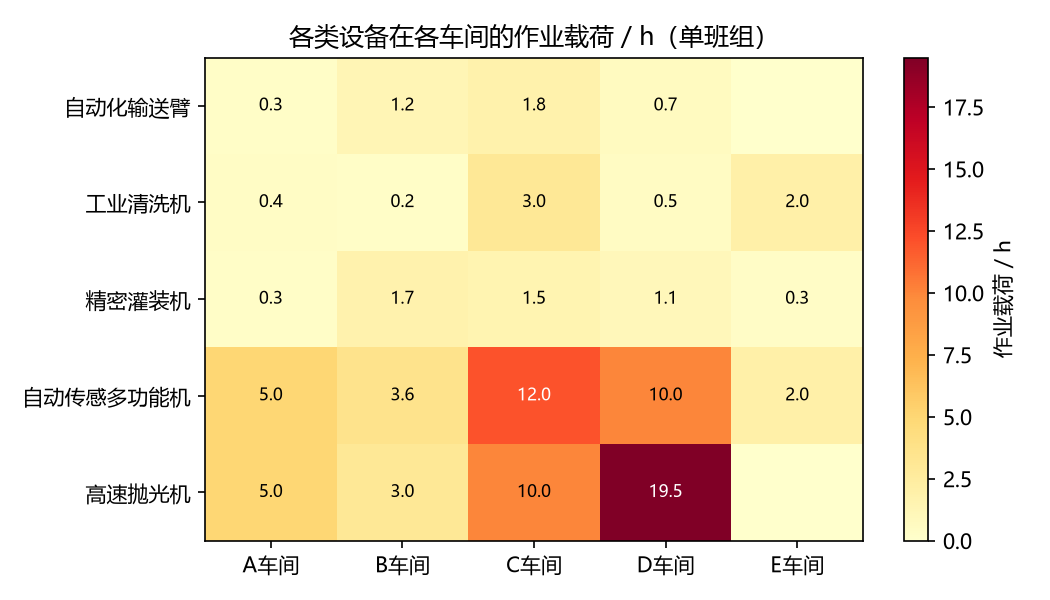
\includegraphics[width=0.72\textwidth]{figs/load_heatmap.png}
\caption{各类设备在各车间的作业载荷热力图（单班组，单位 h）}\label{fig:load}
\end{figure}

\subsection{精确求解与结果}
\noindent\textbf{【编程求解】}\,采用 \texttt{hybrid\_solve.py} 实现混合求解流程，返回 $C_{\max}^{(2)}=144880\,\mathrm{s}$，最优性间隙为零。

其与 $\underline{C}$ 之比为 $1.073$，差额 $9880\,\mathrm{s}$ 来自瓶颈设备跨车间转运与等待。调度甘特图见图~\ref{fig:gq2}，高速抛光机时间轴几乎无空闲。详细调度见表~\ref{tab:q2}。

\begin{figure}[H]
\centering
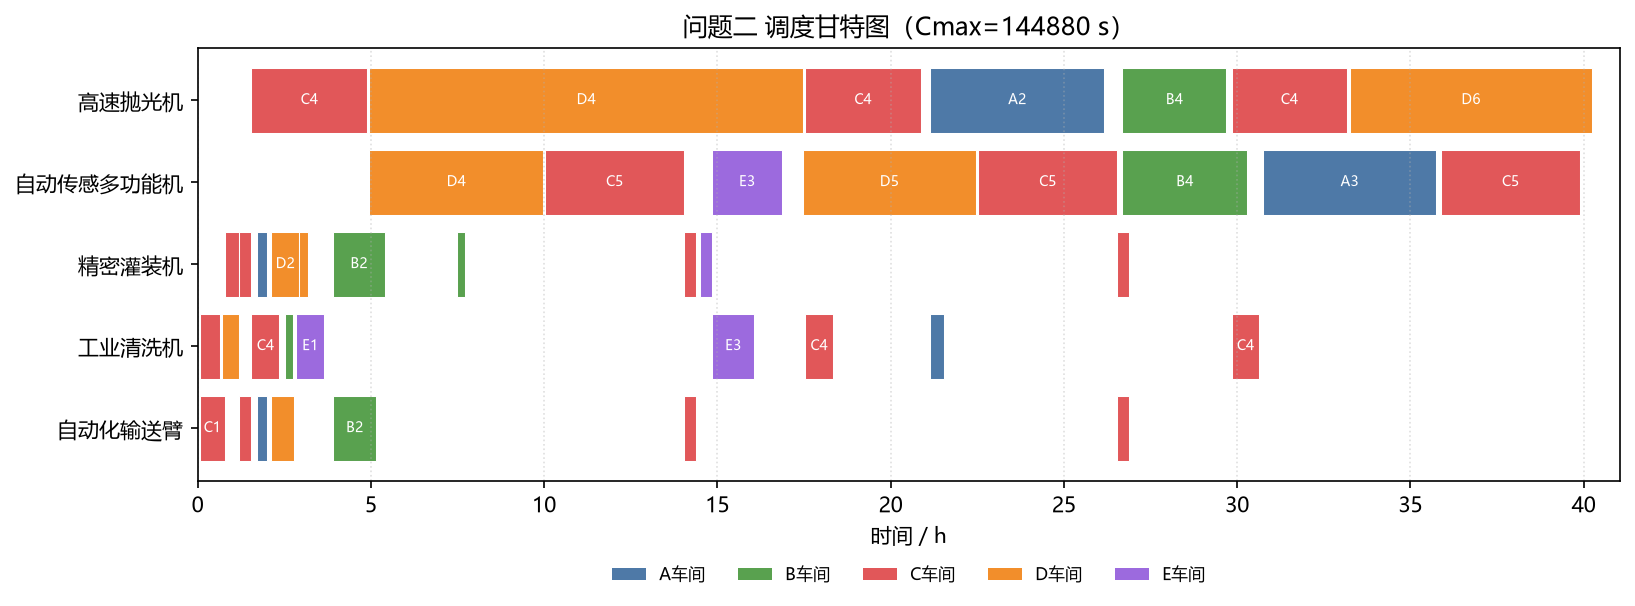
\includegraphics[width=0.95\textwidth]{figs/gantt_q2.png}
\caption{问题二调度甘特图（$C_{\max}=144880\,\mathrm{s}$）}\label{fig:gq2}
\end{figure}

%==================================================================
\section{问题三：双班组资源池化调度模型}

\subsection{建模思路}
问题三在问题二的基础上引入班组 2 的设备。两班组设备类型相同，故自然地将同类设备合并为统一资源池：自动化输送臂 $8$ 台、工业清洗机 $10$ 台、精密灌装机 $10$ 台、自动传感多功能机 $2$ 台、高速抛光机 $2$ 台。模型结构与问题二完全一致，仅两处参数发生变化：其一，工时 $p_{o,r}=\lceil v_o/(e_{o,r}\,n_r^{\text{池}})\cdot3600\rceil$ 中的台数取合并后的池容量，使各工序占用时间相应缩短；其二，初始转运反映两基地协同搬运，首道工序计入 $\max\{\tau_{\mathrm{G1},w},\tau_{\mathrm{G2},w}\}$，即以较远基地的到达时刻为准。该处理保持了与问题二一致的"资源—路由—转运"框架，体现了模型的可扩展性。

\subsection{下界与求解}
资源池化使各类载荷下界减半，瓶颈高速抛光机的载荷下界由 $135000\,\mathrm{s}$ 降至 $67500\,\mathrm{s}$，仍为主导约束。

\noindent\textbf{【编程求解】}\,沿用 \texttt{hybrid\_solve.py}（池化台数与双基地初始转运为参数），由混合求解得
\[
C_{\max}^{(3)}=73575\,\mathrm{s},
\]
并附零间隙最优性证明。其与瓶颈下界之比为 $73575/67500\approx1.090$，超出下界 $6075\,\mathrm{s}$，仍源于瓶颈设备的跨车间转运。相较问题二，双班组使总工期由 $144880\,\mathrm{s}$ 降至 $73575\,\mathrm{s}$，缩短约 $49.2\%$，接近资源翻倍的理想加速比，说明在当前任务结构下并行资源得到了充分利用。调度甘特图见图~\ref{fig:gq3}，详细调度见表~\ref{tab:q3}。

\begin{figure}[H]
\centering
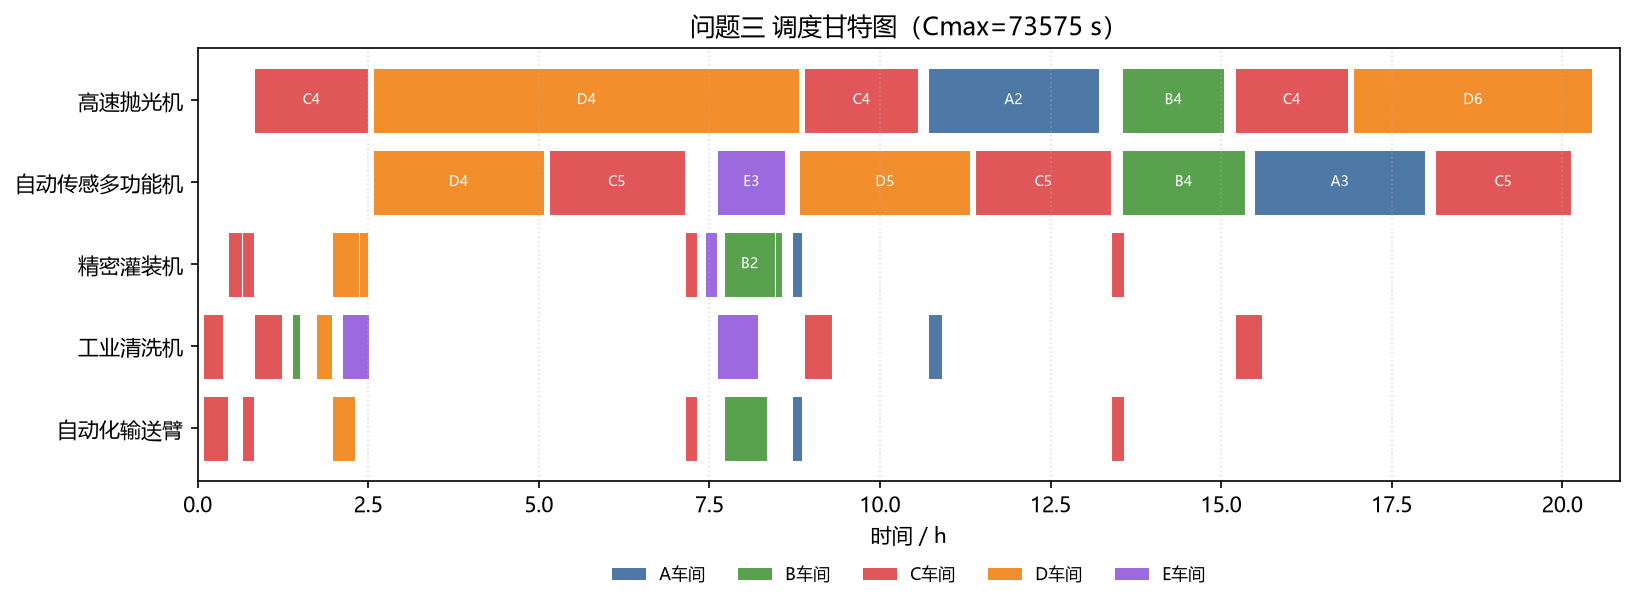
\includegraphics[width=0.95\textwidth]{figs/gantt_q3.png}
\caption{问题三调度甘特图（$C_{\max}=73575\,\mathrm{s}$）}\label{fig:gq3}
\end{figure}

%==================================================================
\section{问题四：预算约束下的购置—调度双层优化模型}

\subsection{购置维度的降维分析}
问题四在双班组基础上追加总额 $500000$ 元的购置预算，需联合确定购置方案与调度策略以最小化总工期。五类设备均可增购，若直接枚举所有组合则维度过高。本文借助资源载荷分析降维：在问题三的池化配置下，仅高速抛光机（载荷下界 $67500\,\mathrm{s}$）与自动传感多功能机（载荷下界 $58680\,\mathrm{s}$）的载荷接近并主导总工期，而输送臂、清洗机、灌装机的载荷不足其三分之一。由于总工期受瓶颈资源载荷下界约束，增购非瓶颈设备无法降低瓶颈载荷，因而不可能改善总工期。据此，购置决策可\emph{严格地}限制在高速抛光机与自动传感多功能机两类，使搜索空间由五维降为二维。

\subsection{双层优化模型}
设增购高速抛光机 $z_{\text{抛}}$ 台、自动传感多功能机 $z_{\text{传}}$ 台，单价分别为 $75000$ 元与 $80000$ 元。模型为
\begin{align}
\min_{z_{\text{抛}},z_{\text{传}}\in\mathbb{Z}_{\ge0}}~~ & C_{\max}^{\ast}\big(n_{\text{抛}}^{\text{池}}+z_{\text{抛}},\ n_{\text{传}}^{\text{池}}+z_{\text{传}}\big) \\
\text{s.t.}~~ & 75000\,z_{\text{抛}} + 80000\,z_{\text{传}} \le 500000,
\end{align}
其中内层 $C_{\max}^{\ast}(\cdot)$ 为给定设备配置下由混合求解（GA/SA 上界 + CP-SAT Hint 证明）所得的最短完工时间。外层枚举购置组合，内层对每个组合调用 \texttt{solve\_hybrid}。

\subsection{求解与结果}
\noindent\textbf{【编程求解】}\,外层枚举、内层混合求解，以"完工时间优先、费用次之"比较。枚举结果显示，最短完工时间随抛光机与传感机的增购显著下降，并在
\[
z_{\text{抛}}=3,\qquad z_{\text{传}}=3
\]
处取得最优，此时购置费用为 $3\times75000+3\times80000=465000\le500000$ 元，对应
\[
C_{\max}^{(4)}=32608\,\mathrm{s}.
\]
该方案使高速抛光机与自动传感多功能机均增至 $5$ 台，瓶颈载荷下界降至 $27000\,\mathrm{s}$，求解所得 $32608\,\mathrm{s}$ 与之比为 $1.207$。相较问题三的 $73575\,\mathrm{s}$，总工期缩短约 $55.7\%$。购置组合对总工期的影响见图~\ref{fig:buy}，可见抛光与传感能力需\emph{均衡}扩充方能最大化收益（如 $z_{\text{抛}}=4,z_{\text{传}}=2$ 费用 $460000$ 元仅得 $36255\,\mathrm{s}$）。购置方案见表~\ref{tab:q5}，调度甘特图见图~\ref{fig:gq4}，详细调度见表~\ref{tab:q4}。

\begin{figure}[H]
\centering
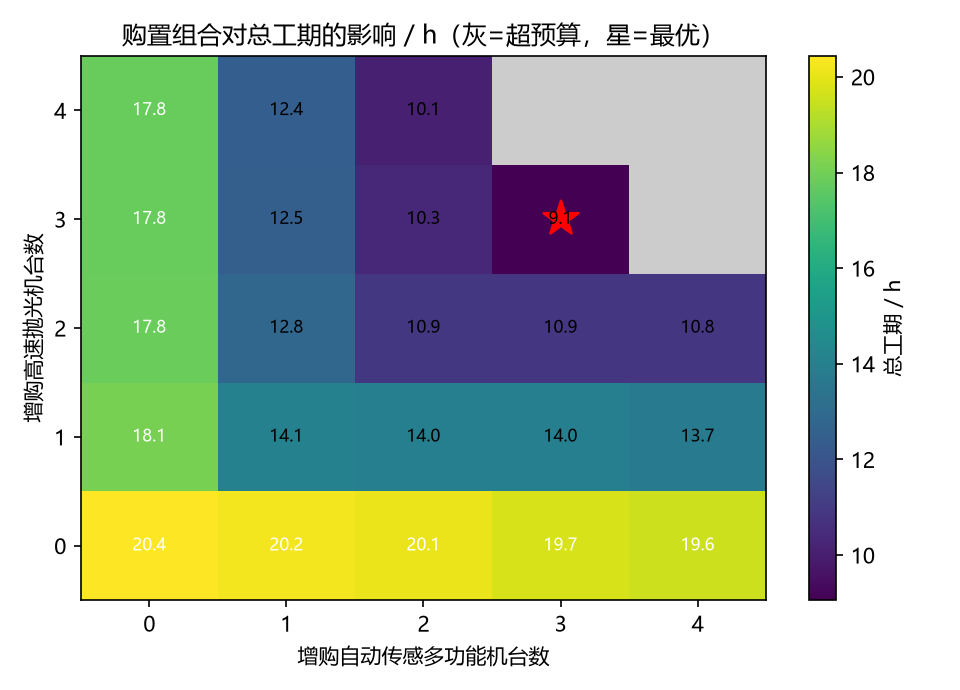
\includegraphics[width=0.62\textwidth]{figs/buy_heatmap.png}
\caption{购置组合对总工期的影响（灰色为超预算，红星为最优方案，单位 h）}\label{fig:buy}
\end{figure}

\begin{figure}[H]
\centering
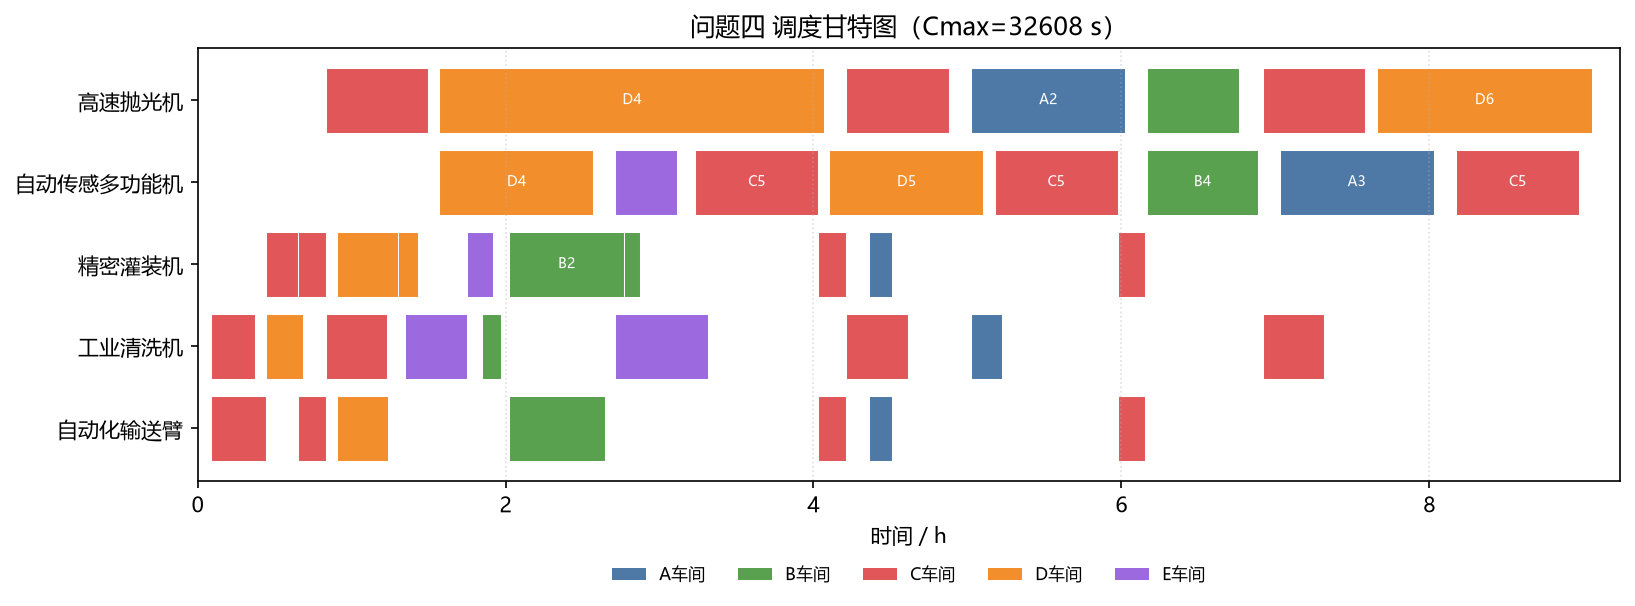
\includegraphics[width=0.95\textwidth]{figs/gantt_q4.png}
\caption{问题四调度甘特图（$C_{\max}=32608\,\mathrm{s}$）}\label{fig:gq4}
\end{figure}

%==================================================================
\section{混合求解结果对照}\label{sec:cv}
问题二至四均采用两层混合求解：GA/SA 生成可行上界，CP-SAT 以 Hint 热启动完成零间隙证明。元启发式解码结果须经独立可行性复核后方纳入对照。

\noindent\textbf{【编程求解】}\,混合求解对照见表~\ref{tab:cv}（\texttt{cross\_validate.py}、\texttt{validate.py}）。

\begin{table}[H]
\centering
\caption{混合求解结果对照（单位 s）}\label{tab:cv}
\begin{tabular}{c c c c c c}
\toprule
问题 & 元启发式上界 & CP-SAT 精确值 & 上界间隙 & 可行性 & 冷/热加速比 \\
\midrule
二 & $144880$ & $144880$ & $0$ & 是 & $1.89$ \\
三 & $73575$ & $73575$ & $0$ & 是 & $1.41$ \\
四 & $32608$ & $32608$ & $0$ & 是 & $2.12$ \\
\bottomrule
\end{tabular}
\end{table}

GA、SA 具有随机性：固定参数下部分种子仍可能停在次优值，但推荐参数下可复现精确最优。本文以 CP-SAT 零间隙证明为最优性依据，元启发式层提供上界与搜索加速。设备利用率见图~\ref{fig:util}。

\begin{figure}[H]
\centering
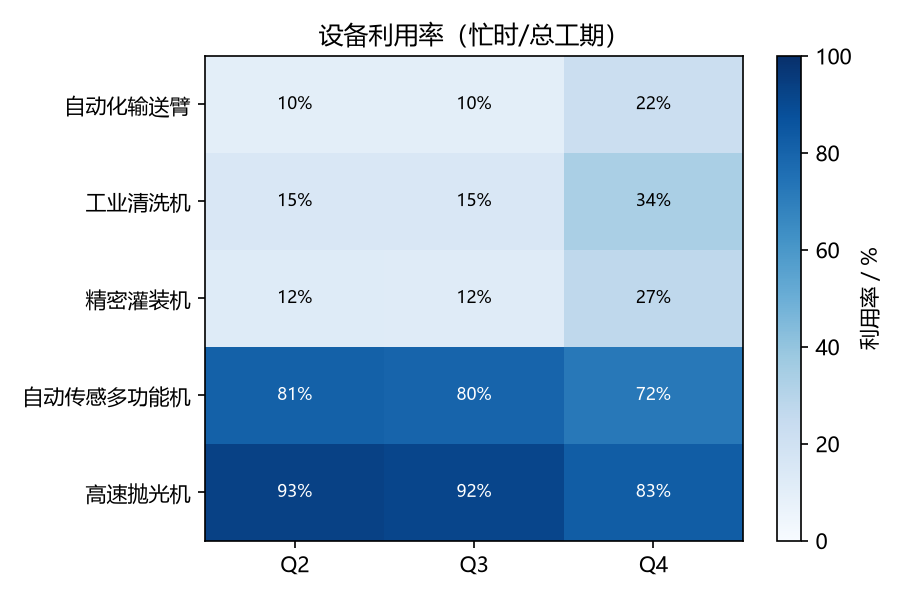
\includegraphics[width=0.6\textwidth]{figs/util_heatmap.png}
\caption{各问设备利用率热力图（忙时/总工期）}\label{fig:util}
\end{figure}

%==================================================================
\section{结果汇总}
四个问题的最短完工时间汇总于表~\ref{tab:summary}。
\begin{table}[H]
\centering
\caption{各问最短完工时间汇总}\label{tab:summary}
\begin{tabular}{c l c c}
\toprule
问题 & 情形 & 最短完工时间 (s) & 备注 \\
\midrule
一 & 班组 1 整修 A 车间 & $37280$ & 解析最优 \\
二 & 班组 1 整修 A--E & $144880$ & 混合求解，零间隙最优 \\
三 & 班组 1、2 整修 A--E & $73575$ & 混合求解，零间隙最优 \\
四 & 预算内购置 $+$ 调度 & $32608$ & 购置费 $465000$ 元，混合求解 \\
\bottomrule
\end{tabular}
\end{table}

%==================================================================
\section{模型评价}
\subsection{模型优点}
其一，本文建立了贯通四问的统一调度框架，以"资源聚合 $+$ 路由转移"将工序时序、协同完工、瓶颈竞争与序列相关转运纳入单一整数规划结构，使四问成为同一模型族在资源容量与决策维度上的递进特例，逻辑连贯、可扩展性强。其二，问题二至四采用 GA/SA 上界生成与 CP-SAT Hint 热启动的两层混合求解，兼顾搜索效率与最优性证明，核心结果均由约束规划给出零间隙证明。其三，每一问均辅以资源载荷下界与关键路径下界，将解与理论下界定量对照，既度量了求解质量，又揭示了"瓶颈设备转运不可避免"这一结构性结论。其四，配备独立于求解器的可行性校验器，对先后、不重叠、转运与双设备完工逐项检查，杜绝"表观最短但不可行"的方案。其五，问题四通过载荷分析将购置维度严格降至瓶颈设备，使双层优化的外层枚举既精简又不失最优性。

\subsection{模型局限与改进方向}
聚合抽象将同类多台设备约束为成组调度，相对允许个体设备在多道并行工序间自由细分的更精细模型略有保守；如 5.5 节所示，在本问题结构下该保守性极小（不超过 $0.16\%$），但在瓶颈设备数量更多、并行机会更丰富的场景中，可进一步建立以累积资源刻画容量、以个体机器刻画路由的精细模型以缩小该间隙。此外，本文假设设备无故障、转运速度恒定，未计入随机扰动；后续可在确定性最优解的基础上引入随机作业时间或转运时间，发展具有鲁棒性的调度策略。

%==================================================================
\appendix
\section{求解程序源代码}\label{app:code}

本附录给出全部求解所用的 Python 程序。程序基于 OR-Tools CP-SAT，以两层混合求解（GA/SA 上界 + CP-SAT Hint 热启动）完成问题二至四。文件清单：\texttt{solver.py}、\texttt{heuristic.py}、\texttt{hybrid\_solve.py}、\texttt{tune\_params.py}、\texttt{extract.py}、\texttt{ga\_q2.py}、\texttt{sa\_q2.py}、\texttt{cross\_validate.py}、\texttt{validate.py}、\texttt{make\_figs.py}。

\begin{table}[H]
\centering
\caption{数据结构与基础参数变量说明}\label{tab:var-data}
\begin{tabular}{p{3.0cm} p{11.5cm}}
\toprule
\textbf{变量名} & \textbf{含义} \\
\midrule
\texttt{TYPES} & 五类设备的键名列表（输送臂/清洗机/灌装机/传感机/抛光机） \\
\texttt{NAME},\,\texttt{PRICE} & 设备键名到中文名称、单价（元/台）的映射 \\
\texttt{G1} & 单班组各类设备台数；\texttt{POOL} 为双班组合并后台数 \\
\texttt{RAW} & 工序原始数据：(编号, 车间, \{类型:(效率,工程量)\}) \\
\texttt{ORDER} & 各车间工序执行顺序（C 车间已含三遍循环） \\
\texttt{DIST} & 班组/车间间距离（米），无向；\texttt{SPEED} 移动速度 $2\,\mathrm{m/s}$ \\
\texttt{trans(w1,w2)} & 由 \texttt{w1} 到 \texttt{w2} 的转运时间 $\lceil d/2\rceil$（同车间为 0） \\
\texttt{build\_ops} & 按设备台数与待修车间生成带工时的工序展开列表 \texttt{ops} 及车间工序链 \texttt{jobs} \\
\bottomrule
\end{tabular}
\end{table}

\begin{table}[H]
\centering
\caption{CP-SAT 调度模型变量说明（\texttt{solve} 函数）}\label{tab:var-model}
\begin{tabular}{p{3.0cm} p{11.5cm}}
\toprule
\textbf{变量名} & \textbf{含义} \\
\midrule
\texttt{counts} & 各类设备总台数（问题一/二取 \texttt{G1}，问题三/四取池化并增购） \\
\texttt{workshops} & 待整修车间集合；\texttt{bases} 初始转运取用的基地集合 \\
\texttt{S[i]},\,\texttt{E[i]} & 工序 $i$ 的开工、完工时刻（秒） \\
\texttt{dur[t]} & 工序对类型 $t$ 的占用时长 $p_{o,t}$ \\
\texttt{arc\_*} & 资源路由布尔变量，对应 $x^{r}_{o,o'}$；\texttt{AddCircuit} 构造单回路 \\
\texttt{init} & 某类设备首道工序的初始转运（双基地取较大值） \\
\texttt{Cmax} & 目标变量，总完工时间；\texttt{solver} 为 CP-SAT 求解器对象 \\
\texttt{hints} & 可选热启动字典（\texttt{starts}、\texttt{cmax}、\texttt{routes}），经 \texttt{AddHint} 注入 \\
\texttt{solve\_time} & CP-SAT 求解耗时（秒）；\texttt{used\_hints} 是否使用热启动 \\
\bottomrule
\end{tabular}
\end{table}

\noindent 下列 \texttt{solver.py} 为 CP-SAT 核心；\texttt{heuristic.py} 为元启发式层；\texttt{hybrid\_solve.py} 为混合求解入口；问题四外层枚举在 \texttt{hybrid\_solve.py} 主程序中实现。

\lstinputlisting[caption={solver.py：CP-SAT 核心（含 hints 热启动）}]{solver.py}
\lstinputlisting[caption={heuristic.py：GA/SA 解码与路由提取}]{heuristic.py}
\lstinputlisting[caption={hybrid\_solve.py：两层混合求解入口}]{hybrid_solve.py}
\lstinputlisting[caption={tune\_params.py：网格调参与冷/热对比}]{tune_params.py}

\noindent 下列 \texttt{extract.py} 用于抽取各问最优解的逐设备调度时间线（生成正文表~\ref{tab:q1}--\ref{tab:q4} 的明细）。

\lstinputlisting[caption={extract.py：调度明细抽取程序}]{extract.py}

\subsection*{混合求解对照与可行性校验}
\noindent\texttt{ga\_q2.py}、\texttt{sa\_q2.py} 调用 \texttt{heuristic.py}。\texttt{validate.py} 为独立可行性校验器。\texttt{cross\_validate.py} 输出混合求解对照表。各文件关键变量见表~\ref{tab:var-heur}。

\begin{table}[H]
\centering
\caption{元启发式与混合求解程序变量说明}\label{tab:var-heur}
\begin{tabular}{p{3.4cm} p{11.1cm}}
\toprule
\textbf{变量/函数} & \textbf{含义} \\
\midrule
\texttt{decode\_full} & 串行调度解码，返回 makespan 与各工序开工时刻 \\
\texttt{extract\_routes} & 由开工时刻反推各资源访问序，生成路由弧 Hint \\
\texttt{run\_metaheuristic} & GA $\rightarrow$ SA 流程，返回上界、starts、耗时 \\
\texttt{solve\_hybrid} & 混合求解入口：元启发式 + 冷/热 CP-SAT \\
\texttt{pox} & 优先保留顺序交叉，保持多重集不变与先后可行 \\
\texttt{neighbor} & 模拟退火邻域：两点交换或单点重插入 \\
\texttt{T0,Tend,alpha,iters} & 模拟退火初温、终温、降温系数、每温迭代次数 \\
\texttt{validate} & 可行性校验，返回 (是否可行, 违规明细, makespan) \\
\bottomrule
\end{tabular}
\end{table}

\lstinputlisting[caption={ga\_q2.py：遗传算法（调用 heuristic）}]{ga_q2.py}
\lstinputlisting[caption={sa\_q2.py：模拟退火（调用 heuristic）}]{sa_q2.py}
\lstinputlisting[caption={validate.py：可行性校验器}]{validate.py}
\lstinputlisting[caption={cross\_validate.py：混合求解结果对照}]{cross_validate.py}

\subsection*{图表生成程序}
\noindent\texttt{make\_figs.py} 调用 \texttt{solver.solve} 取最优调度，生成正文甘特图与热力图。

\lstinputlisting[caption={make\_figs.py：甘特图与热力图生成程序}]{make_figs.py}

%==================================================================
\section{各问结果明细表}

\noindent\textbf{说明：}\,下列各表按设备类型分组给出最优调度。由可分负载假设，同一类型的全部机器成组作业、时间线一致；表中"设备编号"列出该类型参与作业的机器，多台机器在所列时段内同时作业。起始/结束时间为该类设备的作业区间，转运时间体现为相邻作业之间的空档（首道作业前的空档为由基地出发的初始转运）。

% ---------- 表1 Q1 ----------
\begin{longtable}{c p{4.6cm} c c c c}
\caption{问题一结果（班组 1 整修 A 车间，$C_{\max}=37280\,\mathrm{s}$）}\label{tab:q1}\\
\toprule
序号 & 设备编号 & 起始时间 & 结束时间 & 持续(s) & 工序 \\
\midrule
\endfirsthead
\multicolumn{6}{l}{\small 续表~\ref{tab:q1}}\\
\toprule
序号 & 设备编号 & 起始时间 & 结束时间 & 持续(s) & 工序 \\
\midrule
\endhead
\bottomrule
\endfoot
1 & 精密灌装机 1-1$\sim$1-5 & 00:03:20 & 00:21:20 & 1080 & A1 \\
2 & 自动化输送臂 1-1$\sim$1-4 & 00:03:20 & 00:21:20 & 1080 & A1 \\
3 & 高速抛光机 1-1 & 00:21:20 & 05:21:20 & 18000 & A2 \\
4 & 工业清洗机 1-1$\sim$1-5 & 00:21:20 & 00:45:20 & 1440 & A2 \\
5 & 自动传感多功能机 1-1 & 05:21:20 & 10:21:20 & 18000 & A3 \\
\end{longtable}

% ---------- 表2 Q2 ----------
\begin{longtable}{c p{4.6cm} c c c c}
\caption{问题二结果（班组 1 整修 A--E，$C_{\max}=144880\,\mathrm{s}$）}\label{tab:q2}\\
\toprule
序号 & 设备编号 & 起始时间 & 结束时间 & 持续(s) & 工序 \\
\midrule
\endfirsthead
\multicolumn{6}{l}{\small 续表~\ref{tab:q2}}\\
\toprule
序号 & 设备编号 & 起始时间 & 结束时间 & 持续(s) & 工序 \\
\midrule
\endhead
\bottomrule
\endfoot
\multicolumn{6}{l}{\textit{自动化输送臂 1-1$\sim$1-4}}\\
1 & 输送臂 1-1$\sim$1-4 & 00:03:50 & 00:47:02 & 2592 & C1 \\
2 & 输送臂 1-1$\sim$1-4 & 01:11:44 & 01:33:20 & 1296 & C3 \\
3 & 输送臂 1-1$\sim$1-4 & 01:37:40 & 02:17:40 & 2400 & D2 \\
4 & 输送臂 1-1$\sim$1-4 & 02:54:41 & 04:09:41 & 4500 & B2 \\
5 & 输送臂 1-1$\sim$1-4 & 14:15:00 & 14:36:36 & 1296 & C3 \\
6 & 输送臂 1-1$\sim$1-4 & 14:45:21 & 15:03:21 & 1080 & A1 \\
7 & 输送臂 1-1$\sim$1-4 & 26:32:00 & 26:53:36 & 1296 & C3 \\
\midrule
\multicolumn{6}{l}{\textit{工业清洗机 1-1$\sim$1-5}}\\
8 & 清洗机 1-1$\sim$1-5 & 00:03:50 & 00:38:24 & 2074 & C1 \\
9 & 清洗机 1-1$\sim$1-5 & 00:42:44 & 01:11:32 & 1728 & D1 \\
10 & 清洗机 1-1$\sim$1-5 & 01:33:20 & 02:21:20 & 2880 & C4 \\
11 & 清洗机 1-1$\sim$1-5 & 02:30:30 & 02:44:54 & 864 & B1 \\
12 & 清洗机 1-1$\sim$1-5 & 02:50:54 & 03:38:54 & 2880 & E1 \\
13 & 清洗机 1-1$\sim$1-5 & 14:22:06 & 15:34:06 & 4320 & E3 \\
14 & 清洗机 1-1$\sim$1-5 & 17:32:01 & 18:20:01 & 2880 & C4 \\
15 & 清洗机 1-1$\sim$1-5 & 21:00:46 & 21:24:46 & 1440 & A2 \\
16 & 清洗机 1-1$\sim$1-5 & 29:50:20 & 30:38:20 & 2880 & C4 \\
\midrule
\multicolumn{6}{l}{\textit{精密灌装机 1-1$\sim$1-5}}\\
17 & 灌装机 1-1$\sim$1-5 & 00:47:02 & 01:11:44 & 1482 & C2 \\
18 & 灌装机 1-1$\sim$1-5 & 01:11:44 & 01:33:20 & 1296 & C3 \\
19 & 灌装机 1-1$\sim$1-5 & 01:37:40 & 02:25:40 & 2880 & D2 \\
20 & 灌装机 1-1$\sim$1-5 & 02:25:40 & 02:41:06 & 926 & D3 \\
21 & 灌装机 1-1$\sim$1-5 & 02:54:41 & 04:24:41 & 5400 & B2 \\
22 & 灌装机 1-1$\sim$1-5 & 04:24:41 & 04:37:02 & 741 & B3 \\
23 & 灌装机 1-1$\sim$1-5 & 05:51:46 & 06:12:21 & 1235 & E2 \\
24 & 灌装机 1-1$\sim$1-5 & 14:15:00 & 14:36:36 & 1296 & C3 \\
25 & 灌装机 1-1$\sim$1-5 & 14:45:21 & 15:03:21 & 1080 & A1 \\
26 & 灌装机 1-1$\sim$1-5 & 26:32:00 & 26:53:36 & 1296 & C3 \\
\midrule
\multicolumn{6}{l}{\textit{自动传感多功能机 1-1}}\\
27 & 传感机 1-1 & 04:57:40 & 09:57:40 & 18000 & D4 \\
28 & 传感机 1-1 & 10:15:00 & 14:15:00 & 14400 & C5 \\
29 & 传感机 1-1 & 14:22:06 & 16:22:06 & 7200 & E3 \\
30 & 传感机 1-1 & 17:27:40 & 22:27:40 & 18000 & D5 \\
31 & 传感机 1-1 & 22:32:00 & 26:32:00 & 14400 & C5 \\
32 & 传感机 1-1 & 26:41:10 & 30:17:10 & 12960 & B4 \\
33 & 传感机 1-1 & 30:25:40 & 35:25:40 & 18000 & A3 \\
34 & 传感机 1-1 & 35:34:25 & 39:34:25 & 14400 & C5 \\
\midrule
\multicolumn{6}{l}{\textit{高速抛光机 1-1}}\\
35 & 抛光机 1-1 & 01:33:20 & 04:53:20 & 12000 & C4 \\
36 & 抛光机 1-1 & 04:57:40 & 17:27:40 & 45000 & D4 \\
37 & 抛光机 1-1 & 17:32:01 & 20:52:01 & 12000 & C4 \\
38 & 抛光机 1-1 & 21:00:46 & 26:00:46 & 18000 & A2 \\
39 & 抛光机 1-1 & 26:41:10 & 29:41:10 & 10800 & B4 \\
40 & 抛光机 1-1 & 29:50:20 & 33:10:20 & 12000 & C4 \\
41 & 抛光机 1-1 & 33:14:40 & 40:14:40 & 25200 & D6 \\
\end{longtable}

% ---------- 表3 Q3 ----------
\begin{longtable}{c p{4.2cm} c c c c c}
\caption{问题三结果（班组 1、2 整修 A--E，$C_{\max}=73575\,\mathrm{s}$）}\label{tab:q3}\\
\toprule
序号 & 设备编号 & 起始时间 & 结束时间 & 持续(s) & 工序 & 班组 \\
\midrule
\endfirsthead
\multicolumn{7}{l}{\small 续表~\ref{tab:q3}}\\
\toprule
序号 & 设备编号 & 起始时间 & 结束时间 & 持续(s) & 工序 & 班组 \\
\midrule
\endhead
\bottomrule
\endfoot
\multicolumn{7}{l}{\textit{自动化输送臂 1-1$\sim$1-4, 2-1$\sim$2-4}}\\
1 & 输送臂池(8 台) & 00:05:10 & 00:26:46 & 1296 & C1 & 1,2 \\
2 & 输送臂池(8 台) & 00:39:07 & 00:49:55 & 648 & C3 & 1,2 \\
3 & 输送臂池(8 台) & 00:54:15 & 01:14:15 & 1200 & D2 & 1,2 \\
4 & 输送臂池(8 台) & 02:18:52 & 02:56:22 & 2250 & B2 & 1,2 \\
5 & 输送臂池(8 台) & 08:19:55 & 08:30:43 & 648 & C3 & 1,2 \\
6 & 输送臂池(8 台) & 08:54:34 & 09:03:34 & 540 & A1 & 1,2 \\
7 & 输送臂池(8 台) & 13:23:35 & 13:34:23 & 648 & C3 & 1,2 \\
\midrule
\multicolumn{7}{l}{\textit{工业清洗机 1-1$\sim$1-5, 2-1$\sim$2-5}}\\
8 & 清洗机池(10 台) & 00:05:10 & 00:22:27 & 1037 & C1 & 1,2 \\
9 & 清洗机池(10 台) & 00:26:47 & 00:41:11 & 864 & D1 & 1,2 \\
10 & 清洗机池(10 台) & 00:49:55 & 01:13:55 & 1440 & C4 & 1,2 \\
11 & 清洗机池(10 台) & 01:23:05 & 01:30:17 & 432 & B1 & 1,2 \\
12 & 清洗机池(10 台) & 01:36:17 & 02:00:17 & 1440 & E1 & 1,2 \\
13 & 清洗机池(10 台) & 05:12:50 & 05:48:50 & 2160 & E3 & 1,2 \\
14 & 清洗机池(10 台) & 08:53:35 & 09:17:35 & 1440 & C4 & 1,2 \\
15 & 清洗机池(10 台) & 10:42:20 & 10:54:20 & 720 & A2 & 1,2 \\
16 & 清洗机池(10 台) & 15:11:55 & 15:35:55 & 1440 & C4 & 1,2 \\
\midrule
\multicolumn{7}{l}{\textit{精密灌装机 1-1$\sim$1-5, 2-1$\sim$2-5}}\\
17 & 灌装机池(10 台) & 00:26:46 & 00:39:07 & 741 & C2 & 1,2 \\
18 & 灌装机池(10 台) & 00:39:07 & 00:49:55 & 648 & C3 & 1,2 \\
19 & 灌装机池(10 台) & 00:54:15 & 01:18:15 & 1440 & D2 & 1,2 \\
20 & 灌装机池(10 台) & 01:18:15 & 01:25:58 & 463 & D3 & 1,2 \\
21 & 灌装机池(10 台) & 02:00:17 & 02:10:35 & 618 & E2 & 1,2 \\
22 & 灌装机池(10 台) & 02:18:52 & 03:03:52 & 2700 & B2 & 1,2 \\
23 & 灌装机池(10 台) & 08:19:55 & 08:30:43 & 648 & C3 & 1,2 \\
24 & 灌装机池(10 台) & 08:39:53 & 08:46:04 & 371 & B3 & 1,2 \\
25 & 灌装机池(10 台) & 08:54:34 & 09:03:34 & 540 & A1 & 1,2 \\
26 & 灌装机池(10 台) & 13:23:35 & 13:34:23 & 648 & C3 & 1,2 \\
\midrule
\multicolumn{7}{l}{\textit{自动传感多功能机 1-1, 2-1}}\\
27 & 传感机池(2 台) & 02:34:15 & 05:04:15 & 9000 & D4 & 1,2 \\
28 & 传感机池(2 台) & 05:12:50 & 06:12:50 & 3600 & E3 & 1,2 \\
29 & 传感机池(2 台) & 06:19:55 & 08:19:55 & 7200 & C5 & 1,2 \\
30 & 传感机池(2 台) & 08:49:15 & 11:19:15 & 9000 & D5 & 1,2 \\
31 & 传感机池(2 台) & 11:23:35 & 13:23:35 & 7200 & C5 & 1,2 \\
32 & 传感机池(2 台) & 13:32:45 & 15:20:45 & 6480 & B4 & 1,2 \\
33 & 传感机池(2 台) & 15:29:15 & 17:59:15 & 9000 & A3 & 1,2 \\
34 & 传感机池(2 台) & 18:08:00 & 20:08:00 & 7200 & C5 & 1,2 \\
\midrule
\multicolumn{7}{l}{\textit{高速抛光机 1-1, 2-1}}\\
35 & 抛光机池(2 台) & 00:49:55 & 02:29:55 & 6000 & C4 & 1,2 \\
36 & 抛光机池(2 台) & 02:34:15 & 08:49:15 & 22500 & D4 & 1,2 \\
37 & 抛光机池(2 台) & 08:53:35 & 10:33:35 & 6000 & C4 & 1,2 \\
38 & 抛光机池(2 台) & 10:42:20 & 13:12:20 & 9000 & A2 & 1,2 \\
39 & 抛光机池(2 台) & 13:32:45 & 15:02:45 & 5400 & B4 & 1,2 \\
40 & 抛光机池(2 台) & 15:11:55 & 16:51:55 & 6000 & C4 & 1,2 \\
41 & 抛光机池(2 台) & 16:56:15 & 20:26:15 & 12600 & D6 & 1,2 \\
\end{longtable}

% ---------- 表4 Q4 ----------
\begin{longtable}{c p{4.2cm} c c c c c}
\caption{问题四结果（购置后整修 A--E，$C_{\max}=32608\,\mathrm{s}$）}\label{tab:q4}\\
\toprule
序号 & 设备编号 & 起始时间 & 结束时间 & 持续(s) & 工序 & 班组 \\
\midrule
\endfirsthead
\multicolumn{7}{l}{\small 续表~\ref{tab:q4}}\\
\toprule
序号 & 设备编号 & 起始时间 & 结束时间 & 持续(s) & 工序 & 班组 \\
\midrule
\endhead
\bottomrule
\endfoot
\multicolumn{7}{l}{\textit{自动化输送臂 1-1$\sim$1-4, 2-1$\sim$2-4（8 台，未增购）}}\\
1 & 输送臂池(8 台) & 00:05:10 & 00:26:46 & 1296 & C1 & 1,2 \\
2 & 输送臂池(8 台) & 00:39:07 & 00:49:55 & 648 & C3 & 1,2 \\
3 & 输送臂池(8 台) & 00:54:15 & 01:14:15 & 1200 & D2 & 1,2 \\
4 & 输送臂池(8 台) & 03:01:38 & 03:39:08 & 2250 & B2 & 1,2 \\
5 & 输送臂池(8 台) & 04:01:55 & 04:12:43 & 648 & C3 & 1,2 \\
6 & 输送臂池(8 台) & 04:21:28 & 04:30:28 & 540 & A1 & 1,2 \\
7 & 输送臂池(8 台) & 05:58:35 & 06:09:23 & 648 & C3 & 1,2 \\
\midrule
\multicolumn{7}{l}{\textit{工业清洗机 1-1$\sim$1-5, 2-1$\sim$2-5（10 台，未增购）}}\\
8 & 清洗机池(10 台) & 00:05:10 & 00:22:27 & 1037 & C1 & 1,2 \\
9 & 清洗机池(10 台) & 00:26:47 & 00:41:11 & 864 & D1 & 1,2 \\
10 & 清洗机池(10 台) & 00:49:55 & 01:13:55 & 1440 & C4 & 1,2 \\
11 & 清洗机池(10 台) & 01:43:39 & 02:07:39 & 1440 & E1 & 1,2 \\
12 & 清洗机池(10 台) & 02:13:39 & 02:20:51 & 432 & B1 & 1,2 \\
13 & 清洗机池(10 台) & 02:42:50 & 03:18:50 & 2160 & E3 & 1,2 \\
14 & 清洗机池(10 台) & 04:12:43 & 04:36:43 & 1440 & C4 & 1,2 \\
15 & 清洗机池(10 台) & 05:01:28 & 05:13:28 & 720 & A2 & 1,2 \\
16 & 清洗机池(10 台) & 06:55:08 & 07:19:08 & 1440 & C4 & 1,2 \\
\midrule
\multicolumn{7}{l}{\textit{精密灌装机 1-1$\sim$1-5, 2-1$\sim$2-5（10 台，未增购）}}\\
17 & 灌装机池(10 台) & 00:26:46 & 00:39:07 & 741 & C2 & 1,2 \\
18 & 灌装机池(10 台) & 00:39:07 & 00:49:55 & 648 & C3 & 1,2 \\
19 & 灌装机池(10 台) & 00:54:15 & 01:18:15 & 1440 & D2 & 1,2 \\
20 & 灌装机池(10 台) & 01:18:15 & 01:25:58 & 463 & D3 & 1,2 \\
21 & 灌装机池(10 台) & 02:07:39 & 02:17:57 & 618 & E2 & 1,2 \\
22 & 灌装机池(10 台) & 03:01:38 & 03:46:38 & 2700 & B2 & 1,2 \\
23 & 灌装机池(10 台) & 04:01:55 & 04:12:43 & 648 & C3 & 1,2 \\
24 & 灌装机池(10 台) & 04:21:28 & 04:30:28 & 540 & A1 & 1,2 \\
25 & 灌装机池(10 台) & 04:38:58 & 04:45:09 & 371 & B3 & 1,2 \\
26 & 灌装机池(10 台) & 05:58:35 & 06:09:23 & 648 & C3 & 1,2 \\
\midrule
\multicolumn{7}{l}{\textit{自动传感多功能机 1-1, 2-1 $+$ 增购 3 台（共 5 台）}}\\
27 & 传感机池(5 台) & 01:34:15 & 02:34:15 & 3600 & D4 & 1,2 \\
28 & 传感机池(5 台) & 02:42:50 & 03:06:50 & 1440 & E3 & 1,2 \\
29 & 传感机池(5 台) & 03:13:55 & 04:01:55 & 2880 & C5 & 1,2 \\
30 & 传感机池(5 台) & 04:06:15 & 05:06:15 & 3600 & D5 & 1,2 \\
31 & 传感机池(5 台) & 05:10:35 & 05:58:35 & 2880 & C5 & 1,2 \\
32 & 传感机池(5 台) & 06:09:58 & 06:53:10 & 2592 & B4 & 1,2 \\
33 & 传感机池(5 台) & 07:01:40 & 08:01:40 & 3600 & A3 & 1,2 \\
34 & 传感机池(5 台) & 08:10:25 & 08:58:25 & 2880 & C5 & 1,2 \\
\midrule
\multicolumn{7}{l}{\textit{高速抛光机 1-1, 2-1 $+$ 增购 3 台（共 5 台）}}\\
35 & 抛光机池(5 台) & 00:49:55 & 01:29:55 & 2400 & C4 & 1,2 \\
36 & 抛光机池(5 台) & 01:34:15 & 04:04:15 & 9000 & D4 & 1,2 \\
37 & 抛光机池(5 台) & 04:12:43 & 04:52:43 & 2400 & C4 & 1,2 \\
38 & 抛光机池(5 台) & 05:01:28 & 06:01:28 & 3600 & A2 & 1,2 \\
39 & 抛光机池(5 台) & 06:09:58 & 06:45:58 & 2160 & B4 & 1,2 \\
40 & 抛光机池(5 台) & 06:55:08 & 07:35:08 & 2400 & C4 & 1,2 \\
41 & 抛光机池(5 台) & 07:39:28 & 09:03:28 & 5040 & D6 & 1,2 \\
\end{longtable}

% ---------- 表5 Q4 purchase ----------
\begin{table}[H]
\centering
\caption{问题四设备购买情况}\label{tab:q5}
\begin{tabular}{l c c c}
\toprule
设备名称 & 班组 1 购买台数 & 班组 2 购买台数 & 小计 \\
\midrule
自动化输送臂 & 0 & 0 & 0 \\
工业清洗机 & 0 & 0 & 0 \\
精密灌装机 & 0 & 0 & 0 \\
自动传感多功能机 & 2 & 1 & 3 \\
高速抛光机 & 2 & 1 & 3 \\
\midrule
\multicolumn{4}{l}{购买设备总费用：$3\times80000+3\times75000=465000$ 元} \\
\bottomrule
\end{tabular}
\end{table}

\end{document}
